Gestalts- und Volumen- veränderungen können durch das wirken äußerer Kräfte auf einen Körper herbei geführt werden. Die senkrecht zur Oberfläche wirkende Kraft wird als Normalspannung $\sigma$ bezeichnet und steht in linearem Zusammenhang zu der Deformation $\frac {\Delta L}{L}$.

  \begin{equation}
    \sigma = E \cdot \frac{\Delta L}{L}.
    \label{eqn:sigma}
  \end{equation}
Das Hooksche Gesetz \eqref{eqn:sigma} beinhaltet zusätzlich noch den Proportionalitätsfaktor E (Elastizitätsmodul).

\subsection{Einseitige Einspannung}
Durch das wirken einer Kraft F auf einen einseitig eingespannten stabförmigen Probekörper entsteht eine Durchbiegung D(x).
\begin{figure}[h!]
  \centering
  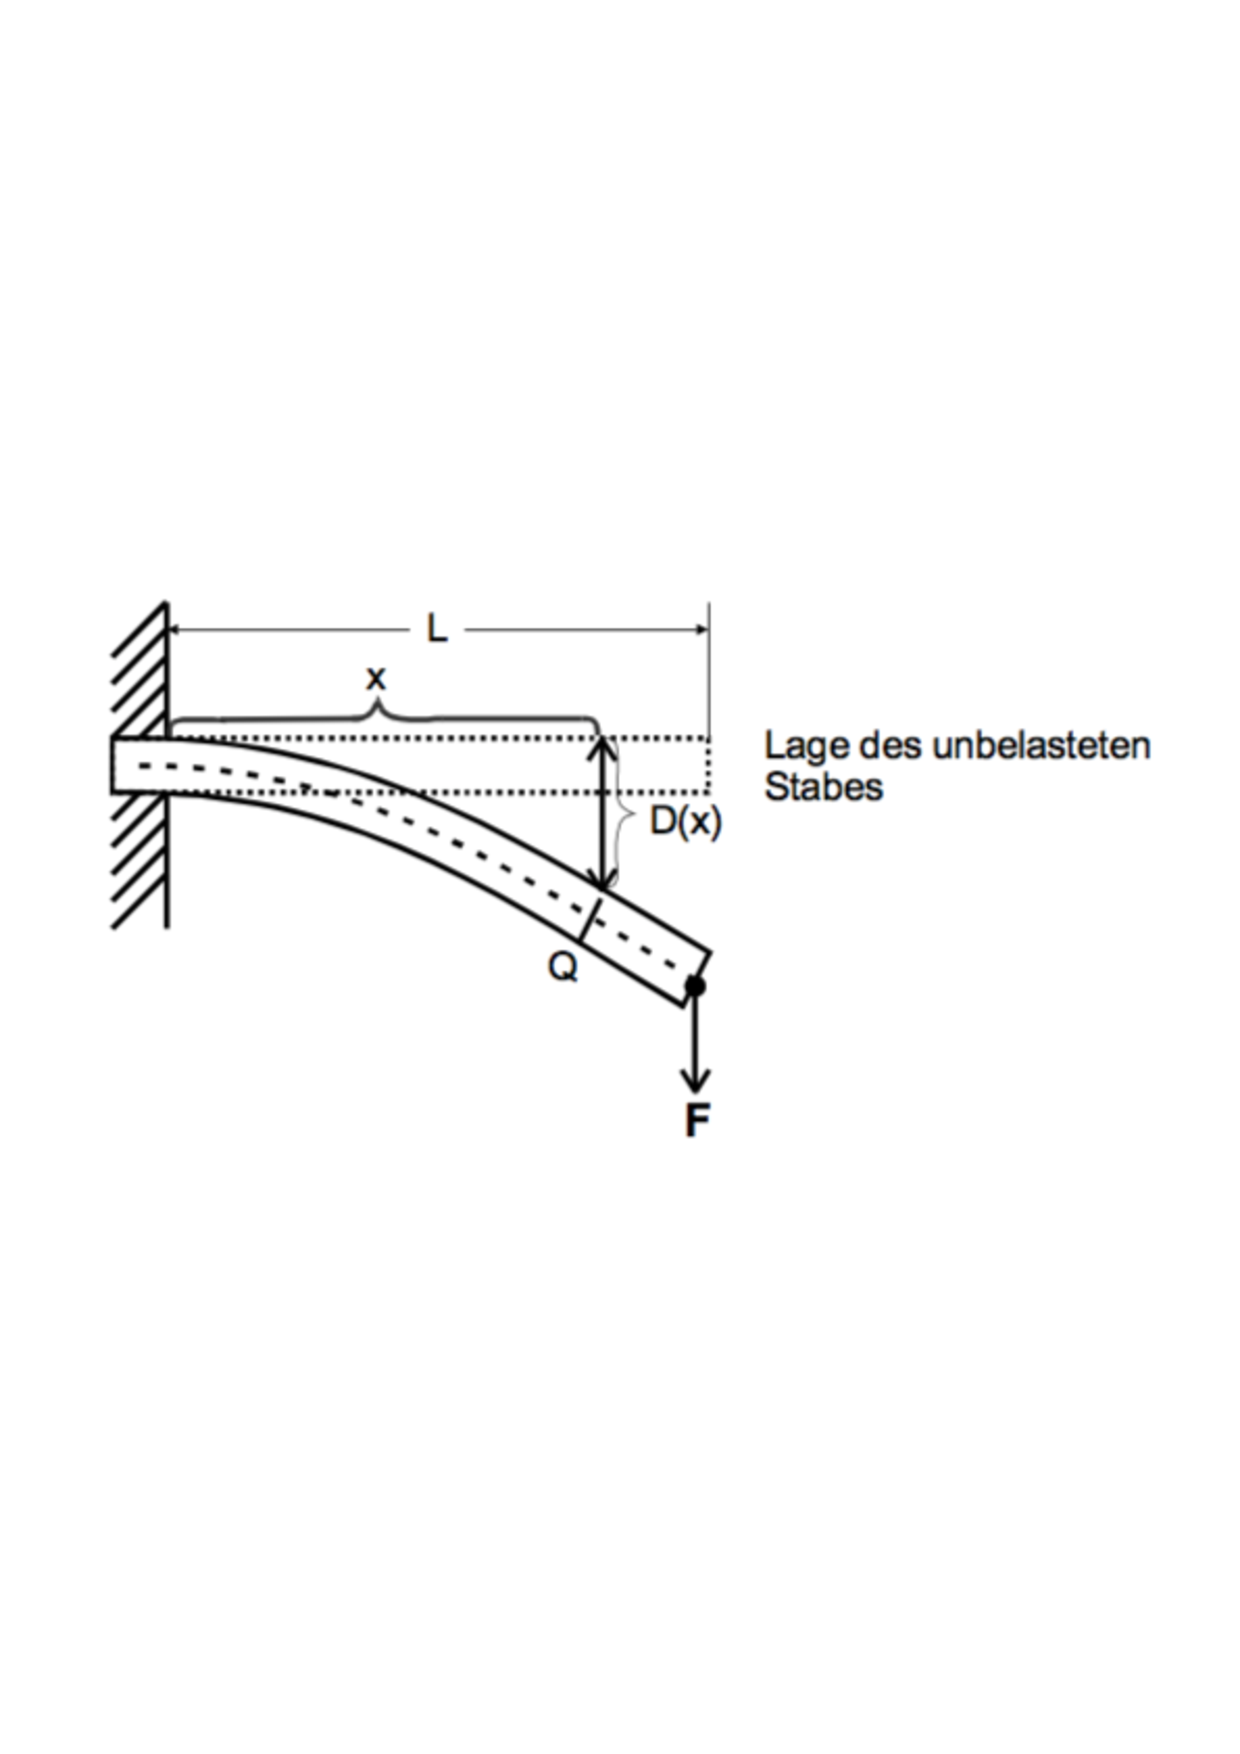
\includegraphics[width=\textwidth]{Durchbiegung.pdf}
  \caption{Durchbiegung eines einseitig eingespannten Stabs \cite{3}}
\end{figure}
\\Im Körper wirken Zug- und Druckspannung entgegen der Kraft F sodass ein Gleichgewicht eintsteht.
\begin{equation*}
  M_F=M_\sigma.
  \label{eqn:Fgl}
\end{equation*}
Das Drehmoment $M_\sigma$ der Spannungen lässt sich über die Integration über den Querschnitt Q bestimmen.

\begin{equation}
  M_\sigma = \int_Q y\sigma(y)dq.
  \label{eqn:int}
\end{equation}
y ist der Abstand des Flächenelements dq, auf welche die Spannung \sigma wirkt, zur neutralen nicht gedehnten Faser.
Das Drehmoment $M_F$ der Kraft F auf das Flächenelement Q lässt sich mit

\begin{equation*}
  M_F=F(L-x).
  \label{eqn:M_F}
\end{equation*}
berechnen. L ist dabei die Länge des Stabes und x der Abstand des Messpunktes zum Anfang des Stabes.
Durch einsetzen in \eqref{eqn:int} ergibt sich nun

\begin{equation}
  \int_Qy \sigma(y)dq=F(L-x).
  \label{eqn:masgl}
\end{equation}
Für $\sigma(y)$ wird das Hooksche Gesetz \eqref{eqn:sigma} verwendet.
Durch einige Überlegungen ergibt sich für $\sigma(y)$ so die Formel

 \begin{equation*}
    \sigma(y) = E y \frac{d^2D}{dx^2}.
    \label{eqn:sigmay}
  \end{equation*}
Durch einsetzen in \eqref{eqn:masgl} ergibt sich

\begin{equation}
  E  \frac{d^2D}{dx^2} \int_Qy^2dq = F(L-x).
  \label{eqn:mom}
\end{equation}
Wobei I mit
\begin{equation}
   I=\int_Qy^2dq.
  \label{eqn:i}
\end{equation}
als Flächenträgheitsmoment berechnet werden kann.
Durch die Integration von \eqref{eqn:mom} ergibt sich

\begin{equation}
  D(x) =     \frac{F}{2EI}(Lx^2-\frac{x^3}{3}).
  \label{eqn:dx}
\end{equation}



\subsection{Zweiseitige Auflage}
Der Stab wird nun auf beiden Seiten aufgelegt.
\begin{figure}
  \centering
  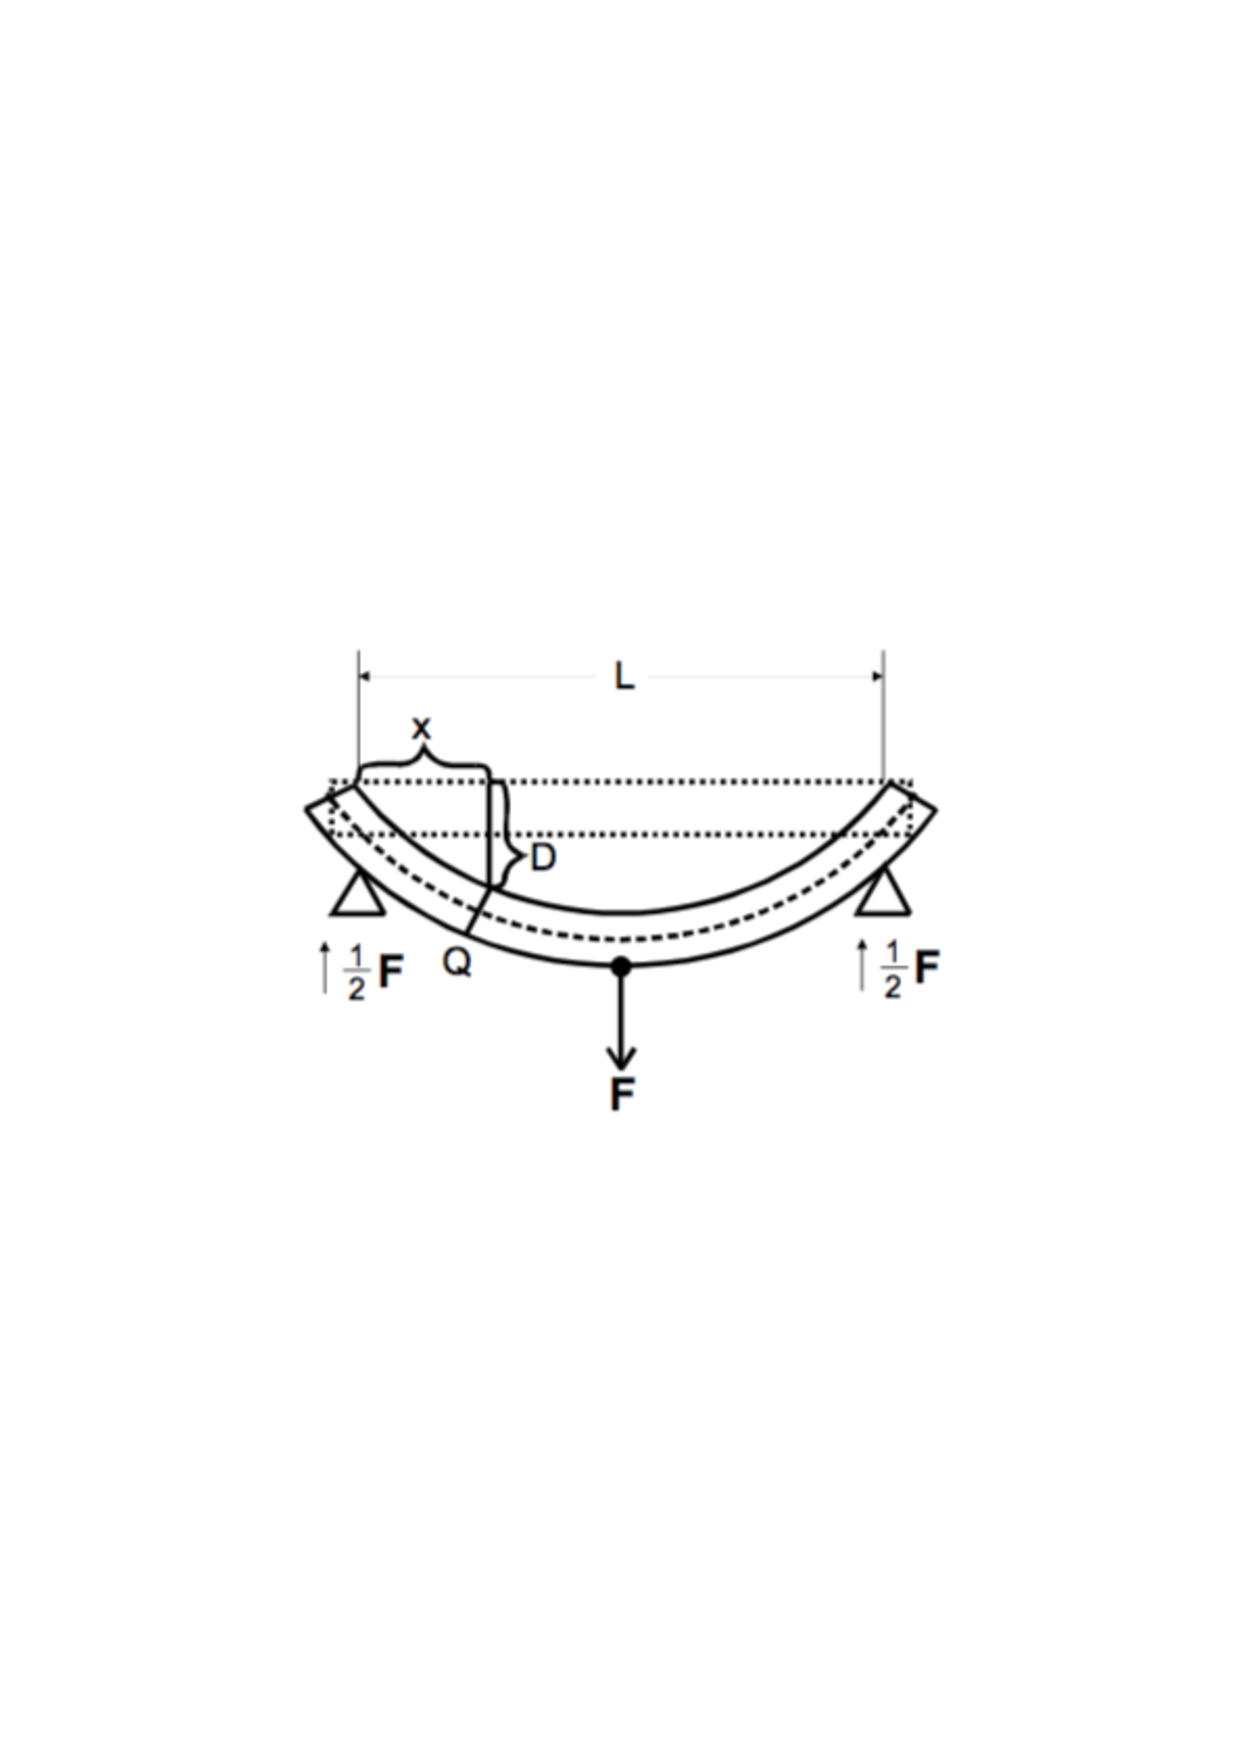
\includegraphics[width=0.8\textwidth]{Durchbiegung2.pdf}
  \caption{Durchbiegung eines beidseitig eingespannten Stabs \cite{3}}
\end{figure}
\\Die Kraft F wirkt daher auf die Mitte das Stabes. Dadurch lässt sich der Stab in zwei Bereiche unterteilen.\\
\begin{itemize}
  \item Der erste Bereich für $0\leq x \leq L/2$
  \item Der zweite Bereich für $L/2 \leq x\leq L$
\end{itemize}
Das Dremoment für den ersten Bereich ist

\begin{equation*}
  M_{F1} = -\frac{f}{2}x.
  \label{eqn:mf1}
\end{equation*}
Für $M_{F2}$ dementsprechend

\begin{equation*}
  M_{F2} = -\frac{F}{2}(L-x).
  \label{eqn:mf2}
\end{equation*}
Durch einsetzten in \eqref{eqn:mom} ergibt sich\\
1.
\begin{equation*}
  \frac{d^2D}{dx^2} = -\frac{F}{EI}\frac{x}{2}.
  \label{eqn:inmom1}
\end{equation*}
2.
\begin{equation*}
  \frac{d^2D}{dx^2} = -\frac{1}{2}\frac{F}{EI}(L-x).
  \label{eqn:inmom2}
\end{equation*}
Nach der Integration haben die Gleichungen die Gestalt\\
1.
\begin{equation*}
  \frac{dD}{dx} = -\frac{F}{EI}\frac{x^2}{4}+C.
  \label{eqn:intmom1}
\end{equation*}
2.
\begin{equation*}
  \frac{D(x)}{dx} = -\frac{1}{2}\frac{F}{EI}(Lx-\frac{x^2}{2})+C´.
  \label{eqn:intmom2}
\end{equation*}

Die Integrationskonstante für C´ hat die Form
\begin{equation*}
  C´  =-\frac{3}{16}\frac{F}{EI}L^2.
  \label{eqn:C`}
\end{equation*}

Für $M_{F1}$ ergibt sich durch eine weitere Integration die Formel
\begin{equation}
  D(x) = \frac{F}{48EI}(3L^2x-4x^3).
  \label{eqn:D(x)1}
\end{equation}

$M_{F2}$ hat mit C´ dann die Form
\begin{equation}
  D(x) = \frac{F}{48EI}(4x^3-12Lx^2+9L^2x-L^3).
  \label{eqn:D(x)2}
\end{equation}

%\subsection{Allgemeine Theorie}
%
%  \begin{equation}
%    \sigma = E \cdot \frac{\delta L}{L}.
%
%
%  \end{equation}
%  \label{eqn:???}
%
